\documentclass[12pt,a4paper]{article}

\usepackage[T1,T2A]{fontenc}
\usepackage[utf8]{inputenc}
\usepackage[english,russian]{babel}
\usepackage{microtype}
\usepackage{csquotes}
\usepackage{amsmath}
\usepackage{amsthm}
\usepackage{amssymb}
\usepackage{mathtext}
\usepackage{physics}
\usepackage{newfloat}
\usepackage{caption}
\usepackage{indentfirst}
\usepackage{titlesec,titletoc}
\usepackage{geometry}
\usepackage{hyperref}
\usepackage{mdframed}
\usepackage[inline]{enumitem}
\usepackage{graphicx}
\usepackage{subfig}
\usepackage[titletoc,toc]{appendix}

\DeclareGraphicsExtensions{.pdf,.png,.jpg,.PNG}
\graphicspath{{./img/}}
\captionsetup[figure]{justification=centering}
\renewcommand{\thesubfigure}{\asbuk{subfigure}}
\DeclareCaptionLabelSeparator{dotseparator}{. }
\captionsetup{labelsep=dotseparator}
\geometry{left=1cm,right=1cm,top=2cm,bottom=2cm}
\makeatletter\appto{\appendices}{\def\Hy@chapapp{Appendix}}\makeatother
\renewcommand{\appendixtocname}{Приложения}
\renewcommand{\appendixpagename}{Приложения}

\DeclareMathOperator{\Rot}{\mathbf{rot}}
\DeclareMathOperator{\Grad}{\mathbf{grad}}
\DeclareMathOperator{\Div}{\mathbf{div}}
\DeclareMathOperator{\D}{D}
\newcommand{\V}[1]{\mathbf{#1}}
\newcommand{\Op}[1]{\hat{\V{#1}}}


\title{Сферические гармоники}
\author{Василевский А.В.}

\begin{document}

    \maketitle
    \tableofcontents

    %
    %
    %
    %%%%%%%%%%%%%%%%%%%%%%%%%%%%%%%%%%%%%%%%%%%%%%%%%%%%%%%%%%%%%%%%%%%%%%%
    %                           SECTION                                   %
    %%%%%%%%%%%%%%%%%%%%%%%%%%%%%%%%%%%%%%%%%%%%%%%%%%%%%%%%%%%%%%%%%%%%%%%
    %
    %
    %

    \section*{Введение}

        Целью данной работы является построение мод электромагнитного поля в сферическом резонаторе.

        Классические методики решения данной задачи в значительной степени эвристичны, другие приводят к весьма громоздким результатам. К тому же их применение к полям б\'{о}льшей тензорной размерности весьма проблематично.

        В данной работе приводится новый подход, в основе которого лежат векторы Киллинга пространства, в котором распространяется поле. Данный подход учитывает естественную симметрию объемлющего пространства, тем самым требует более коротких выкладок. К тому же он естественным образом обобщается для описания полей любой тензорной размерности, например гравитационного.

        Впервые указанная методика была применена для описания полей различной тензорной размерности на трехмерной сфере \cite{burlankov_tmf}.

    %
    %
    %
    %%%%%%%%%%%%%%%%%%%%%%%%%%%%%%%%%%%%%%%%%%%%%%%%%%%%%%%%%%%%%%%%%%%%%%%
    %                           SECTION                                   %
    %%%%%%%%%%%%%%%%%%%%%%%%%%%%%%%%%%%%%%%%%%%%%%%%%%%%%%%%%%%%%%%%%%%%%%%
    %
    %
    %

    \section{Уравнение на сферические моды}

        Уравнение на сферические моды получается из волнового уравнения, которое, в свою очередь, получается из стационарных уравнений Максвелла в среде.

        В изотропной немагнитной среде, где справедливо $\V{D} = \varepsilon \V{E}$, волновое уравнение для вектора $\V{E}$ принимает вид:
        %
        \begin{equation}\label{eq:wave_equation}
            \Delta \V{E} = - \varepsilon \frac{\omega^2}{c^2} \V{E} .
        \end{equation}
        %
        Оно является уравнением на собственные функции и собственные значения (моды) оператора Лапласа $\Delta$, что позволяет эффективно применить аппарат теории операторов для его решения.

        В задаче о сферическом резонаторе спектр мод дискретен и определяется двумя числами, $l$ и $m$, т.е. общее решение уравнения \autoref{eq:wave_equation} выражается через линейную комбинацию полученных мод: $\V{E} = \sum a_{l,m} \V{E}_{l,m}$.

    %
    %
    %
    %%%%%%%%%%%%%%%%%%%%%%%%%%%%%%%%%%%%%%%%%%%%%%%%%%%%%%%%%%%%%%%%%%%%%%%
    %                           SECTION                                   %
    %%%%%%%%%%%%%%%%%%%%%%%%%%%%%%%%%%%%%%%%%%%%%%%%%%%%%%%%%%%%%%%%%%%%%%%
    %
    %
    %

    \section{Методика нахождения сферических мод}

        В \cite{math_appendix} были введены операторы повышения $\Op{l}_{+} = \Op{l}_x - i \Op{l}_y$ и понижения $\Op{l}_{-} = \Op{l}_x + i \Op{l}_y$, чье действие на некоторую моду $h_{l, m}$ описывается следующими выражениями:
        %
        \begin{equation}\begin{aligned}
            \Op{l}_{+} h_{l, m} &= h_{l, m+1} , \\
            \Op{l}_{-} h_{l, m} &= h_{l, m-1} ,
        \end{aligned}\end{equation}
        %
        причем $- l \le m \le l$, т.е. существует такое предельное значение $m = \pm l$, при котором
        %
        \begin{equation}\begin{aligned}
            \Op{l}_{+} h_{l, l}   &= 0 , \\
            \Op{l}_{-} h_{l, - l} &= 0 .
        \end{aligned}\end{equation}
        %
        Это означает, что из некоторой произвольной моды $h_{l, m}$ можно получить другую моду $h_{l, n}$ последовательным применением операторов $\Op{l}_{+}$ или $\Op{l}_{-}$ необходимое количество раз.

        Наиболее интересной является базовая мода, т.е. мода с $m = 0$, для которой
        %
        \begin{equation}
            \Op{l}_z h_{l, 0} = 0 .
        \end{equation}
        %
        В \cite{math_appendix} был получен явный вид векторов Киллинга евклидова пространства в контравариантном виде в сферических координатах, в частности вектора $\V{l}_z$:
        %
        \begin{equation}
            \V{l}_z = \qty{ 0, 0, 1 } = \V{e}_\varphi .
        \end{equation}
        %
        Подействуем оператором
        %
        \begin{equation}
            \Op{l}_z
                = \partial_{\V{l}_z}
                = {\V{l}_z}^i \pdv{x^i}
                = \pdv{\varphi}
        \end{equation}
        %
        на $h_{l, 0}$:
        %
        \begin{equation}
            \Op{l}_z h_{l, 0} = \pdv{h_{l, 0}}{\varphi} = 0 ,
        \end{equation}
        %
        откуда видно, что базовая мода $h_{l, 0}$ не зависит от $\varphi$.

        Зависимость базовой моды от $\theta$ определяется из следующего уравнения:
        %
        \begin{equation}\label{eq:basemode_op_eq}
            \Op{l}^2 h_{l, 0}
                = \qty( \Op{l}_{+} \Op{l}_{-} + \Op{l}_z^2 - i \Op{l}_z ) h_{l, 0}
                = \Op{l}_{+} \Op{l}_{-} h_{l, 0}
                = - l (l + 1) h_{l, 0}
        \end{equation}
        %
        или эквивалентного ему
        %
        \begin{equation}
            \Op{l}^2 h_{l, 0}
                = \qty( \Op{l}_{-} \Op{l}_{+} + \Op{l}_z^2 + i \Op{l}_z ) h_{l, 0}
                = \Op{l}_{-} \Op{l}_{+} h_{l, 0}
                = - l (l + 1) h_{l, 0} .
        \end{equation}

        Зависимость от $r$, т.е. радиальная часть $h_{l, m}$, определяется из уравнения \autoref{eq:wave_equation}.

        Отсюда вытекает следующая методика построения сферических мод:
        %
        \begin{enumerate}[noitemsep]
            \item Построение базовых мод с $m = 0$ и определенным $l$;
            \item Нахождение радиальных функций для базовых мод;
            \item Получение остальных $2l$ производных мод с $m = \pm 1, \pm 2, \dots$ путем применения операторов повышения и понижения.
        \end{enumerate}

    %
    %
    %
    %%%%%%%%%%%%%%%%%%%%%%%%%%%%%%%%%%%%%%%%%%%%%%%%%%%%%%%%%%%%%%%%%%%%%%%
    %                           SECTION                                   %
    %%%%%%%%%%%%%%%%%%%%%%%%%%%%%%%%%%%%%%%%%%%%%%%%%%%%%%%%%%%%%%%%%%%%%%%
    %
    %
    %

    \section{Нахождение угловых частей сферических мод}

        Найдем угловые части сферических мод.

        Ранее было показано, что базовая мода не зависит от координаты $\varphi$. Операторы вращений не содержат дифференцирования по $r$ и действуют на каждую из контравариантных координат моды независимо. Поэтому здесь мы ограничимся рассмотрением скалярной моды $f_{l,m}(\theta, \varphi)$.

        Расписывая \autoref{eq:basemode_op_eq} применительно к базовой моде $f_{l,0}(\theta) \equiv f_l(\theta)$ в явном виде, получим
        %
        \begin{equation}
            f_l''(\theta) + f_l'(\theta) \cot \theta + l (l + 1) f_l(\theta) = 0 .
        \end{equation}
        %
        Данное уравнение определяет два решения: $P$- и $Q$-полиномы Лежандра. Вторые, однако, обращаются в бесконечность при значении параметра $\theta = 0, \pi$. Поэтому базовая мода без учета нормировки равна
        %
        \begin{equation}
            f_l(\theta) = P_l\qty(\cos \theta)
        \end{equation}
        %
        Можно показать, что оператор повышения порядка $m$, применяемый к некоторой функции одной переменной $f(\theta)$, имеет вид
        %
        \begin{equation}\begin{aligned}
            \Op{l}^m_{+} f(\theta)
                &= \qty(
                    \underbrace{\Op{l}_{+} \dots \Op{l}_{+}}_{\text{$m$ раз}}
                ) f(\theta) \\
                &= i^m \exp(- i m \varphi) \qty(
                    (-1)^m \sin^m \theta \dv[m]{f\qty(\cos\theta)}{\qty(\cos\theta)}
                ) .
        \end{aligned}\end{equation}
        %
        Для $P$-полиномов Лежандра присоединенные $P$-полиномы Лежандра определяются следующим образом:
        %
        \begin{equation}
            P^m_l(\cos\theta) = (-1)^m \sin^m \theta \dv[m]{P_l\qty(\cos\theta)}{\qty(\cos\theta)} ,
        \end{equation}
        %
        откуда видно, что
        %
        \begin{equation}
            f_{l,m}(\theta,\varphi)
                = \Op{l}^m_{+} f_l(\theta)
                = i^m \exp(- i m \varphi) P^m_l\qty(\cos\varphi) .
        \end{equation}

        На \autoref{fig:angle_modes} представлено несколько угловых мод $f_{l,m}(\theta,\varphi)$.
        %
        \begin{figure}[h]
            \centering
            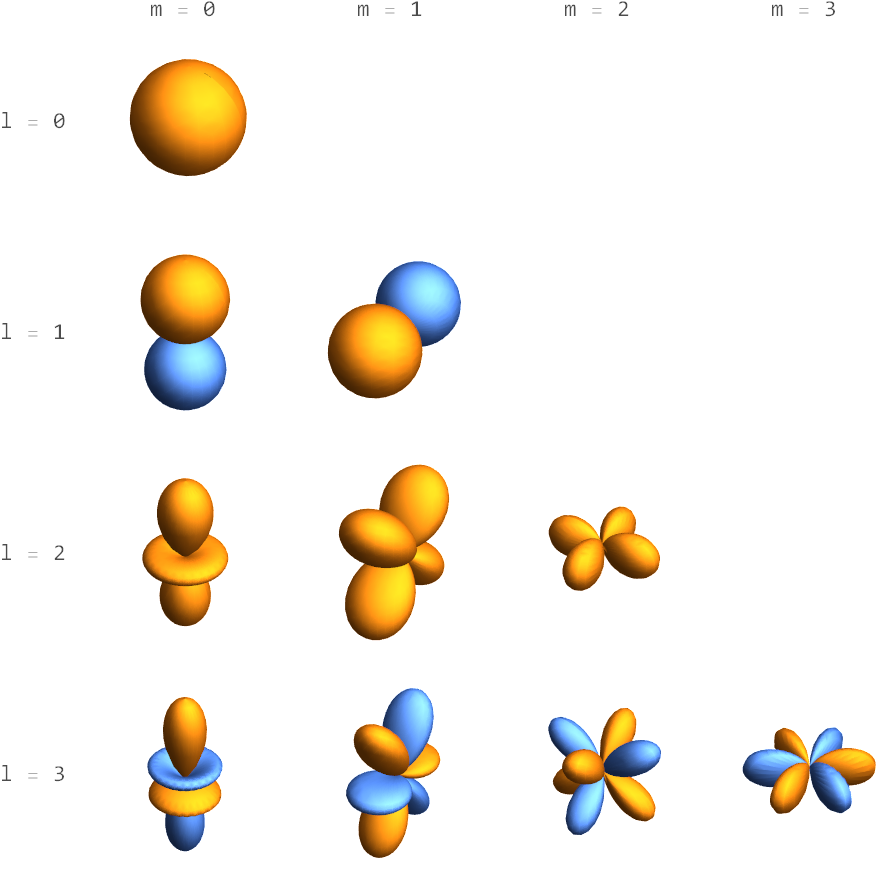
\includegraphics[width=0.5\textwidth]{angle_modes}
            \caption[]{Сферические угловые моды для нескольких $l$}
            \label{fig:angle_modes}
        \end{figure}

    %
    %
    %
    %%%%%%%%%%%%%%%%%%%%%%%%%%%%%%%%%%%%%%%%%%%%%%%%%%%%%%%%%%%%%%%%%%%%%%%
    %                        BIBLIOGRAPHY                                 %
    %%%%%%%%%%%%%%%%%%%%%%%%%%%%%%%%%%%%%%%%%%%%%%%%%%%%%%%%%%%%%%%%%%%%%%%
    %
    %
    %

    \nocite{*}
    \bibliographystyle{../../lib/doc/bib/utf8gost705s}
    \bibliography{../../lib/doc/bib/physics,math}

\end{document}
